% !TEX TS-program = xelatex
% !TEX encoding = UTF-8

% This is a simple template for a XeLaTeX document using the "article" class,
% with the fontspec package to easily select fonts.

\documentclass[11pt]{report} % use larger type; default would be 10pt
\usepackage{fontspec} % Font selection for XeLaTeX; see fontspec.pdf for documentation
\defaultfontfeatures{Mapping=tex-text} % to support TeX conventions like ``---''
\usepackage{xunicode} % Unicode support for LaTeX character names (accents, European chars, etc)
\usepackage{xltxtra} % Extra customizations for XeLaTeX
\fontspec{"[DroidSerif.ttf]"}
\setmainfont{Droid Serif} % set the main body font (\textrm), assumes Charis SIL is installed
%\setsansfont{Deja Vu Sans}
%\setmonofont{Deja Vu Mono}
\usepackage{amsmath}
\usepackage{xfrac,unicode-math}
\setmathfont[version=cambria]{Cambria Math}
\mathversion{cambria}
\usepackage{cleveref}
% other LaTeX packages.....
\usepackage{geometry} % See geometry.pdf to learn the layout options. There are lots.
\geometry{letterpaper} % or letterpaper (US) or a5paper or....
%\usepackage[parfill]{parskip} % Activate to begin paragraphs with an empty line rather than an indent

\usepackage{graphicx} % support the \includegraphics command and options

\title{237D Fusion Technology \\
Handout v. 1.1}
\author{Professor Mohamed Abdou}
%\date{} % Activate to display a given date or no date (if empty),
         % otherwise the current date is printed 


\begin{document}
\maketitle
\chapter{Incentives for Developing Fusion}
\label{intro}
This handout is intended for students who have some prior knowledge of nuclear science. There are shorthand notations used in this handout with which we assume the student has some familiarity. It is highly recommended that the student be comfortable with the material of Chapter 3 from Introduction to Nuclear Engineering by John R. Lamarsh. Some fundamentals of the kinematics of nuclear reactions, etc. are covered there and not explicitly discussed here.
 
\subsection*{Incentives for Developing Fusion}
\begin{enumerate}
\item Inexhaustible energy source
\item Potential environmental and safety advantages
\item Reasonable economics
\end{enumerate}


\subsection*{Fission Process}
\begin{itemize}
\item Splitting of a heavy nucleus into two lighter ones plus two or three neutrons
\item Conversion of mass into KE
\end{itemize}


\subsection*{Fusion Process}
\begin{itemize}
\item Two light nuclei join (fuse) together to form a heavier and lighter one
\item Conversion of mass into KE
\item Energy appears as KE of reaction products
\end{itemize}



\subsection{Mass defect and binding energy}
The mass of a nucleus is less than the sum total mass of all its nucleons (neutrons, N, and protons, Z). This difference is called ``mass defect'' and can be used to find the binding energy (neglecting the binding energy of electrons),
\begin{align}
\mathrm{BE} &= \left[Zm_H + Nm_n - m(A,Z)\right]c^2\\
\cfrac{BE}{A}&=\cfrac{BE}{Z+N}
\end{align}

In fission, we have reactions such as...
\begin{equation}
^{235}\mathrm{U}+~_0^1\mathrm{n} \rightarrow \mathrm{X}_1 +\mathrm{ X}_2 + \nu
\end{equation}
The binding energy of neutrons in uranium is liberated when it is captured. It provides internal energy for two lighter elements,
\begin{equation}
\mathrm{m}(U) + \mathrm{m}(n) \rightarrow \mathrm{m}(X_1) + \mathrm{m}(X_2) + \mathrm{m}(\nu)
\end{equation}
This energy liberated is the gain from fission.

In fusion, two nuclei fuse to form a heavier one, {\it e.g.} the deuterium-deuterium reaction has two, nearly equally probable, reactions
\begin{equation}
\mathrm{D} +~\mathrm{D}\xrightarrow{}~_1^1\mathrm{H}+~\mathrm{T}
\end{equation}
or sometimes
\begin{equation}
\mathrm{D} +~\mathrm{D}\xrightarrow{}~\mathrm{n}+~^3_2\mathrm{He}
\end{equation}
How much energy is released from this fusion? From the binding energy equation above, we calculate
\begin{align*}
BE &= \left[2(\text{mass of $_1^2$H}) - (\text{mass of $_1^1$H} + \text{mass of $_1^3$H})\right]c^2\\
& = 4.05~\text{MeV}
\end{align*}
and
\begin{align*}
BE &= \left[2m(_1^2\mathrm{H}) - m(_0^1\mathrm{n}) - m(_2^3\mathrm{He})\right]c^2\\
& = 3.27~\text{MeV}
\end{align*}

There are other possible fusion reactions of interest, they're listed here along with their liberated energy.
\begin{align}
\mathrm{D} +~\mathrm{T}&\xrightarrow{}~^4\mathrm{He}+\mathrm{n}+17.58~\text{MeV} \label{eq:DT}\\
\mathrm{D} +~^3\mathrm{He}&\xrightarrow{}~^4\mathrm{He}+~\mathrm{H}+~18.34\text{MeV}\label{eq:D3He}\\
\mathrm{H} +~^6\mathrm{Li}&\xrightarrow{}~^4\mathrm{He}+~^3\mathrm{He}+4~\text{MeV}\\
\mathrm{T} +~\mathrm{T}&\xrightarrow{}~\mathrm{n}+\mathrm{n}+~^4\mathrm{He}+11.3~\text{MeV}\\
\mathrm{p} +~\mathrm{B}^{11}&\xrightarrow{}3~_2^4\mathrm{He}+8.68~\text{MeV}
\end{align}

\subsection{Considerations in selecting a fuel cycle}
\begin{itemize}
\item High reaction probability
\item High energy yield
\item Availability of fuel
\item Reaction products are manageable and ``harmless''
\end{itemize}

\begin{figure}
\centering
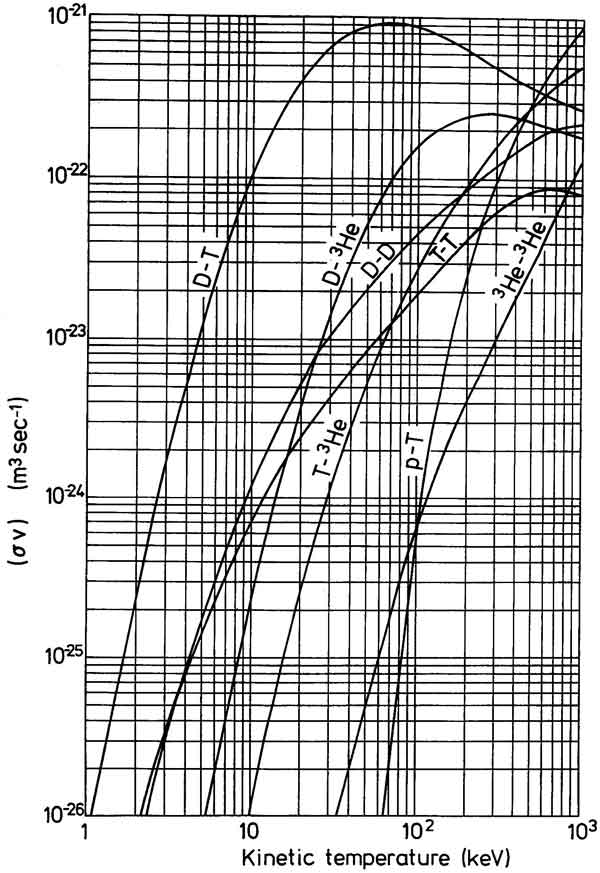
\includegraphics[width=0.75\textwidth]{../images/fusion_rxnrates.jpg} 
\caption{Reaction probabilities for some light-element fusion reactions}
\label{fig:fusion_rxnrates}
\end{figure}

From reaction probability curves of Fig.~\ref{fig:fusion_rxnrates}, we note:
\begin{itemize}
\item D-T has the highest reaction probability
\item D-T requires the lowest ion temperature (easier heating technology)
\item Reactions other than D-T require much higher ion temperature
\item Reactions other than D-T have lower reaction probability
\end{itemize}


Therefore we're left with the following reactions of interest
\begin{align}
\mathrm{D} +~\mathrm{T}&\xrightarrow{}~^4\mathrm{He}+\mathrm{n}\\
\mathrm{D} +~\mathrm{D}&\xrightarrow{}~_1^1\mathrm{H}+~\mathrm{T}\\
\mathrm{D} +~\mathrm{D}&\xrightarrow{}~\mathrm{n}+~^3_2\mathrm{He}\\
\mathrm{D} +~^3\mathrm{He}&\xrightarrow{}~^4\mathrm{He}+~\mathrm{H}
\end{align}

A neutron-free reaction ({\it i.e.} no neutrons in the reaction products) are very desirable but it will be a long time before we realize them. More information on fuel cycles can be found in textbooks by Gross (chapter 2) and Dolan (chapter 1).

\section{Fuel availability, D-T}
Here we'll focus on the availability of fuel for the D-T reaction, given in Eq.~\ref{eq:DT}

\subsection{Deuterium}
Deuterium, $D$, or $^2H$, is a stable isotope and occurs in the natural hydrogen of water in an average abundance of 0.015 mole percent. As an example there is 1 part D in every 6670 hydrogen atoms.  $D_2O$ is often referred to as `heavy water'.

{\it Example}: From the natural abundance of D, in 1 m$^3$ of ocean water, we find that there is $8\times 10^{12}$ joules of energy from D. This is equivalent to energy from about 1360 barrels of oil or 270 tons of coal. The world's ocean volume is approximately $1.5\times 10^{18}$ m$^3$. This translates into $5\times 10^{13} $ tons of deuterium available on Earth. This is an enormous amount! Commercial methods of extracting deuterium from water are available.

\subsection{Tritium}
Tritium is radioactive with a half life of only about 12.32 years. It is a $\beta^-$ emitter (no $\gamma$ rays). Owing to its short half life, it is not available in nature. Because of this, we need to generate it somehow if it is to be used in a D-T fusion reactor so that the reaction is self-sufficient. Fortunately, this can be achieved. When natural lithium interacts with a neutron, its two most common isotopes have the following reaction

\begin{align}
\mathrm{n} + ~^7\mathrm{Li} &\xrightarrow ~\mathrm{n}+\alpha + \mathrm{T} -2.47~\text{MeV}\label{eq:Li7T}\\
\mathrm{n} + ~^6\mathrm{Li} &\xrightarrow ~ \alpha + \mathrm{T} +4.78~\text{MeV} \label{eq:Li6T}
\end{align}
Note that here we've used the common short-hand of $\alpha$ in place of the helium nucleus. Therefore if we use the neutron from the D-T reaction to interact with lithium, we would have an inexhaustible energy source (to the extent of lithium and deuterium availability, which are abundant).


\subsection{Lithium}

Natural lithium occurs with the isotopic abundances of 92.58\% for $^7Li$ and 7.42\% for $^6Li$. Lithium metal is soft, has a low density (of 0.53 g/cm$^3$), and has a physical appearance similar to lead. The average abundance of lithium in the Earth's crust is approximately 65 parts per million by weight. The concentration of lithium in sea water is also about 0.17 g/m$^3$. Lithium reserves are estimated to be sufficient for the United States' electrical demand for more than 600 years.

\section{Fuel availability, D-$^3$He}
Here we focus on the availability of the D-$^3$He reaction, given in Eq.~\ref{eq:D3He}.

\subsection{Helium-3}
Helium-3 is a scarce material, its natural abundance on Earth is 0.00013\%. Though there are several means of producing it, namely

\begin{align}
\mathrm{H}(^6\mathrm{Li},~^4\mathrm{He})~^3\mathrm{He}\\
\mathrm{D}(\mathrm{D},\mathrm{n})~^3\mathrm{He}\\
\mathrm{D}(^6\mathrm{Li},\mathrm{n})~^3\mathrm{He}+\alpha
\end{align}
Note we've now used the common shorthand for representing reactions. Write these out long-hand on your own.

Another alternative is to simply produce tritium (as discussed above) and then let it $\beta$-decay, as
\begin{equation}
\mathrm{T} \xrightarrow{}~^3\mathrm{He} + \beta^-
\end{equation}

In all the methods described above, there are difficulties in the production of helium-3. Alternatively, there have been suggestions to retrieve the element from the moon, where it was found to be relatively abundant.

\section{Elementary introduction to fusion reactors}
In this section we provide a very brief introduction into many of the components and features of a fusion reactor. All the components are shown together schematically in Fig.~\ref{fig:reactor_components}.
\subsection{Plasma}
Plasma is the fourth state of matter. It consists of ionized atoms (ions) and free electrons. This state of matter is uncommon on Earth but it's the dominant state of matter in the Universe: the stars and much of interstellar space. In the plasma is where energy is produced and fuel is consumed in the fusion reactor.
\subsection{Plasma heating system}
On Earth, to heat a plasma to thermonuclear temperatures, we have several means, such as:
\begin{itemize}
\item Energetic particle (D) beams
\item RF waves
\item Ohmic heating
\end{itemize}


\subsection{Magnets}\label{sec:magnets}
Plasma in a reactor is basically gas at high temperature, equivalent to 100 million degrees. It can not be contained in standard ways with conventional materials. One approach to confining the plasma is via strong magnetic fields manipulating the ionized particles of the plasma. A specific style of magnetic confinement developed by Soviet physicists is with a `tokamak' device. The tokamak is the confinement approach of many current research plasma devices as well as the ITER experiment - though there are other magnetic confinement styles (stellerators, for one) and other confinement techniques (such as inertial confinement). In a tokamak reactor, there are two main groups of super-conducting magnets: toroidal and polodial.

Roughly speaking, a measure of the efficiency of magnetic confinement is often given as a `beta factor'. This is defined as the ratio of plasma pressure to magnetic pressure (in other words, plasma thermal energy to magnetic field energy). 
\begin{equation}
\beta = \cfrac{\text{plasma pressure}}{\text{magnetic pressure}}
\end{equation}

The $\beta$ value is not constant throughout the volume of the confinement region, though an average $\beta$ is often given. A high plasma pressure is desired to maintain high temperatures and relates to the yield of the fusion reactor. At the same time, the cost of super-conducting magnetics increases as the magnetic pressure increases so that term relates to the amount of `cost' of maintaining the plasma. Therefore, to maintain an economical fusion reactor a high-beta value is necessary.

\subsection{Vacuum}
For a fusion reactor, we need to keep background pressure very low. To accomplish this, the entire plasma system must be kept inside of a vacuum vessel.

\subsection{Plasma ash removal (impurity control)}
For proper operation, we must remove the plasma ash products ($\alpha$s in the D-T cycle). The removal is done via a limiter or divertor. The products are pumped out with a vacuum system. The materials considered for a divertor are Be, C, or W. As of this writing, ITER is going forward with tungsten divertors.

\subsection{First Wall}
The components directly facing the plasma that are responsible for removing a large portion of the plasma heat load are collectively known as the `first wall'. The first wall (FW) is exposed to the high energy neutrons originating in the plasma as well as the radiation heat flux. The FW experiences extremely high mechanical and electromagnetic loadings. The FW is a critical component because on top of satisfying thermal and mechanical performance requirements, for maintaining safety, the materials chosen for the FW must also have low activation.

\subsection{Blanket}
The complex structure that surrounds, or `covers' the plasma chamber behind the first wall is called the blanket. The blanket is responsible for energy conversion (absorbing neutron energy and surface heat flux) and breeding tritium. Tritium breeding is done with lithium as described with Eqns.~\ref{eq:Li7T} and~\ref{eq:Li6T}.

\subsection{Radiation Shield}
A shield is necessary to protect magnets and other components as well as protecting personnel operating the fusion reactor from neutrons not absorbed by the blanket.

\subsection{Heat transport system}
Finally, a system is necessary to transport heat from the fusion reactor into a standard steam turbine system for electricity generation.
\begin{figure}
\centering
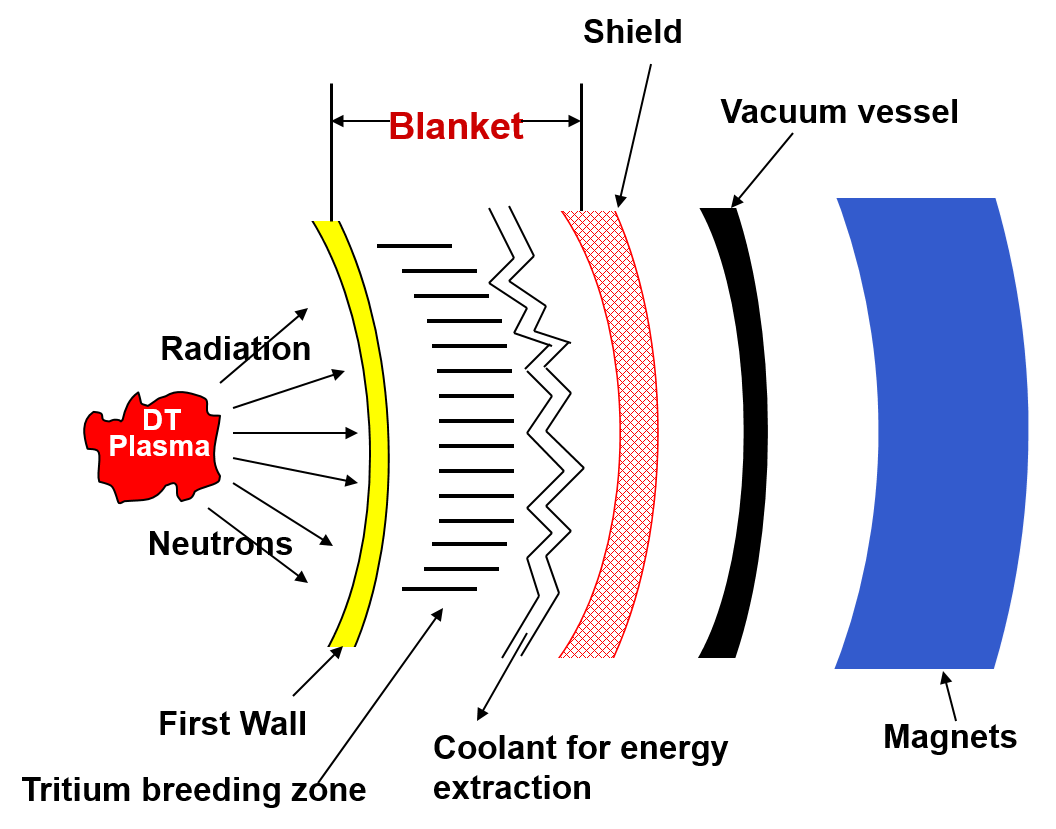
\includegraphics[width=\textwidth]{../images/reactor_components.png} 
\caption{Sketch showing the locations of different reactor components surrounding a plasma}
\label{fig:reactor_components}
\end{figure}
\section{Reaction summary}
Table~\ref{tab:reactions1} summarizes many of the power reactions discussed in this handout. Numbers in parenthesis are the approximate energies of individual reaction products. Table~\ref{tab:reactions2} summarizes the tritium breeding nuclear reactions.
\begin{table}
    \begin{tabular}{lllll}
     \vspace{0.5em}name       & fusion reaction                               & abbreviated form            & MeV   & joule            \\ \hline \vspace{-0.7em}\\
    \vspace{0.5em}DT         & D + T $\rightarrow~_2^4$He (3.52) + $~_0^1$n(14.1)  &  T(d,n)$^4$He               & 17.59 &$2.818\times10^{-12}$ \\
    \vspace{0.5em}DDn        & D + D $\rightarrow~_2^3$He (0.82) + $~_0^1$n(2.45) & D(d,n)$^3$He             & 3.27  & $5.24\times10^{-13}$ \\
    \vspace{0.5em}DDp        & D + D $\rightarrow~$T (1.01) + p (3.02)                       & D(d,p)T                     & 4.03  &$6.46\times10^{-13}$  \\
\vspace{0.5em}    TT         & T + T $\rightarrow~_2^4$He + $~_0^1$n+ $~_0^1$n & T(t,2n)$^4$He           & 11.3  &  $1.81\times10^{-12}$ \\
\vspace{0.5em}    D-$^3$He & D + $~_2^3$He $\rightarrow~_2^4$He (3.66) + p(14.6) &$^3$He(d,p)$^4$He     & 18.3  & $2.93\times10^{-12}$ \\
\vspace{0.5em}     p-$^6$Li & p + $~_3^6$Li $\rightarrow~_2^4$He  + $~_2^3$He & $^6$Li(p,$\alpha$)$^3$He & 4.02  &$6.44\times10^{-13}$ \\
\vspace{0.5em}   p-$^{11}$B & p + $~_5^{11}$B $\rightarrow~3$($_2^4$He)  & $^{11}$B(p,2$\alpha$)$^4$He & 8.68  & $1.39\times10^{-12}$   \\
    \end{tabular}\caption{Fusion reactions of interest for power generation}\label{tab:reactions1}
\end{table}

\begin{table}
    \begin{tabular}{lllll}
     \vspace{0.5em}name       & fusion reaction                               & abbreviated form            & MeV   & joule            \\ \hline\vspace{-0.7em}\\
    \vspace{0.5em}n-$^6$Li & n$_\text{thermal}$ + $~_3^6$Li $\rightarrow~_2^4$He(2.05)  + T(2.73) & $^6$Li(n,$\alpha$)T & 4.78  &$7.66\times10^{-13}$ \\
    \vspace{0.5em}n-$^7$Li & n$_\text{fast}$ + $~_3^7$Li $\rightarrow~_2^4$He  + T + n & $^7$Li(n,n'$\alpha$)T & -2.47  &$-3.96\times10^{-13}$
    \end{tabular}\caption{Fusion reactions of interest for tritium breeding}\label{tab:reactions2}
\end{table}

\section{Review of Important Parameters}
We define the fusion power, $P_f$, as the power released in a differential volume of plasma, dV. Using definitions of nuclear reaction rates, this power is written as
\begin{equation}\label{eq:fusion-power-integral}
P_f = \int\!n_Dn_T\langle\sigma v\rangle_{DT} E_{DT}\,\mathrm{d}V
\end{equation}
where $E_{DT} = 17.6$ MeV (remember: MeV can be translated as an energy value, find the conversion of this into J for SI units). Then we assume an equal partition of tritium and deuterium atomic densities, in other words $n_D = n_T = \frac{n}{2}$ where $n = n_D + n_T$. The above then becomes
\begin{equation}\label{eq:virginFusionPower}
P_f =\int\!\cfrac{n^2}{4}\langle\sigma v\rangle_{DT} E_{DT} \,\mathrm{d}V
\end{equation}

We can find the atomic density in terms of the plasma pressure which is itself a sum of the partial pressure of electrons, ions, $\alpha$ particles, and other impurities;
\begin{equation}\label{eq:plasmapressure}
p = n_ekT_e + n_ikT_i + n_\alpha kT_\alpha + \dots
\end{equation}

Consider the case where there's a much smaller $\alpha$ particle density than other ions $n_\alpha \ll n_i$. For a DT reaction, we can assume the ion and electron densities are equal, $n_e = n_i = n$. Thus
\begin{align}
p &= n\left(kT_e + kT_i\right)\nonumber\\
n & = \cfrac{p}{kT_e + kT_i}
\end{align}

While there are spatial variations in all of these terms, for this discussion we assume they are average values throughout the volume so we can then write the fusion power as
\begin{align}\label{eq:fusion-power}
P_f & =\cfrac{\langle\sigma v\rangle_{DT} E_{DT}}{4}\left( \cfrac{p}{kT_e + kT_i}\right)^2 V\nonumber\\
P_f & = \cfrac{\langle\sigma v\rangle_{DT}}{(kT_i)^2\left(1 + \frac{T_e}{T_i}\right)^2}~\cfrac{p^2E_{DT}}{4}\,V
\end{align}

Viewing \Cref{eq:fusion-power}, we make the important distinction that fusion power maximizes when the term $\frac{\langle\sigma\nu\rangle}{T^2}$ is maximized, not simply the reaction rate, $\langle \sigma \nu \rangle$, alone - as you might assume from \Cref{eq:fusion-power-integral}. Assuming that value is maximized and set, we analyze the second term in the fusion power equation. To do this, we introduce the $\beta$ term described in Sec.~\ref{sec:magnets}. As mentioned it is the ratio of plasma to magnetic pressure, but we now define it in engineering terms. The magnetic pressure is in terms of the permeability of free space, $\mu_0$, and the magnetic flux density, $B$.
\begin{equation}
p_\text{mag} = B^2/2\mu_0
\end{equation}

The plasma pressure is given in Eq.~\ref{eq:plasmapressure}. Combining these gives the beta value of:
\begin{equation}
\beta = \frac{P_\text{kinetic}}{P_\text{mag}} = \cfrac{n_ekT_e + n_ikT_i + n_\alpha kT_\alpha + \dots}{B^2/(2\mu_0)}
\end{equation}

{\it Discussion}: Show that after introducing $\beta$, and assuming that $T_e = T_i = T$, into the fusion power equation, we find
\begin{equation}\label{eq:fusionPower}
P_f = C\beta^2B^4\cfrac{\langle\sigma v\rangle_{DT}}{T^2}E_{DT}V
\end{equation}

Finally from the form of Eq.~\ref{eq:fusionPower}, we can see that the power of a fusion reactor is proportional to 
\begin{itemize}
\item $\beta^2$, or magnetic confinement efficiency 
\item $B^4$, or technology limits
\item $\cfrac{\langle\sigma v\rangle}{T^2}$, or fuel cycle cross-sections
\item $E$, or the energetics of the chosen fuel cycle
\end{itemize} 



\section{Wall loads}
Here we'll discuss the loads associated with individual products of a fusion reaction. We continue to assume the DT reaction of Eq.~\ref{eq:DT} whose power is given by Eq.~\ref{eq:virginFusionPower}. We define the parameter, $S$:
\begin{equation}
S_T =\cfrac{\text{the number of neutrons}}{\text{second of time $\times$ unit volume of plasma}} = \cfrac{n^2}{4}\,\langle\sigma v\rangle
\end{equation}
Then the total number is simply
\begin{equation}
S_T =\cfrac{\text{total number of neutrons}}{\text{second of plasma}} = \cfrac{n^2}{4}\,\langle\sigma v\rangle\, V = \int S(\vec{r})\,\mathrm{d}\vec{r} = \int \frac{n^2}{4}\langle\sigma\nu\rangle\,\mathrm{d}\vec{r}
\end{equation}

The number of DT reactions is equal to the number of neutrons emitted.

We can now define a {\emph current} of virgin ({\it i.e.} uncollided) fusion neutrons to the first wall as

\begin{align}
J & = \text{virgin neutron current to the first wall}\nonumber\\
& = \text{ Number of neutrons passing through the first wall per unit area}\nonumber\\
& = \cfrac{S_T}{A_w}
\end{align}
where $A_w$ is the first wall surface area.

The neutron wall load, $P_{nw}$ is then defined as

\begin{align}
P_{nw} & = \text{Fusion neutron power incident on the first wall per unit area}\nonumber\\
& = JE_0
\end{align}
where $E_0$ is the energy carried per fusion neutron (which we recall is 14.06 MeV for a DT reaction)

Then the total fusion neutron power is simply the neutron wall load multiplied by the surface area of the first wall
\begin{align}
P_f &= P_{nw}A_w\\
P_f & = S_T E_0
\end{align}

In other words, 

\begin{equation}
P_f = P_{nw}\cfrac{17.58}{14.06}
\end{equation}
for a DT reaction. A typical range for neutron wall load in commercial fusion reactor design is to anticipate $P_{nw} \in (1,5)$ MW/m$^2$.

We now consider the partitioning of powers in a power plant. We have the following short list of major powers to consider
\begin{itemize}
\item $P_i$, input power (from {\it e.g.} current drive) which should be generally small
\item $P_{nw}$, neutron power to the wall
\item $P_\alpha$, $\alpha$ particle power (and other charged particles) incident mainly on the divertor
\item $P_{rad}$, radiated power from the plasma onto the FW (bremsstrahlung radiation)
\end{itemize}
\begin{figure}
\centering
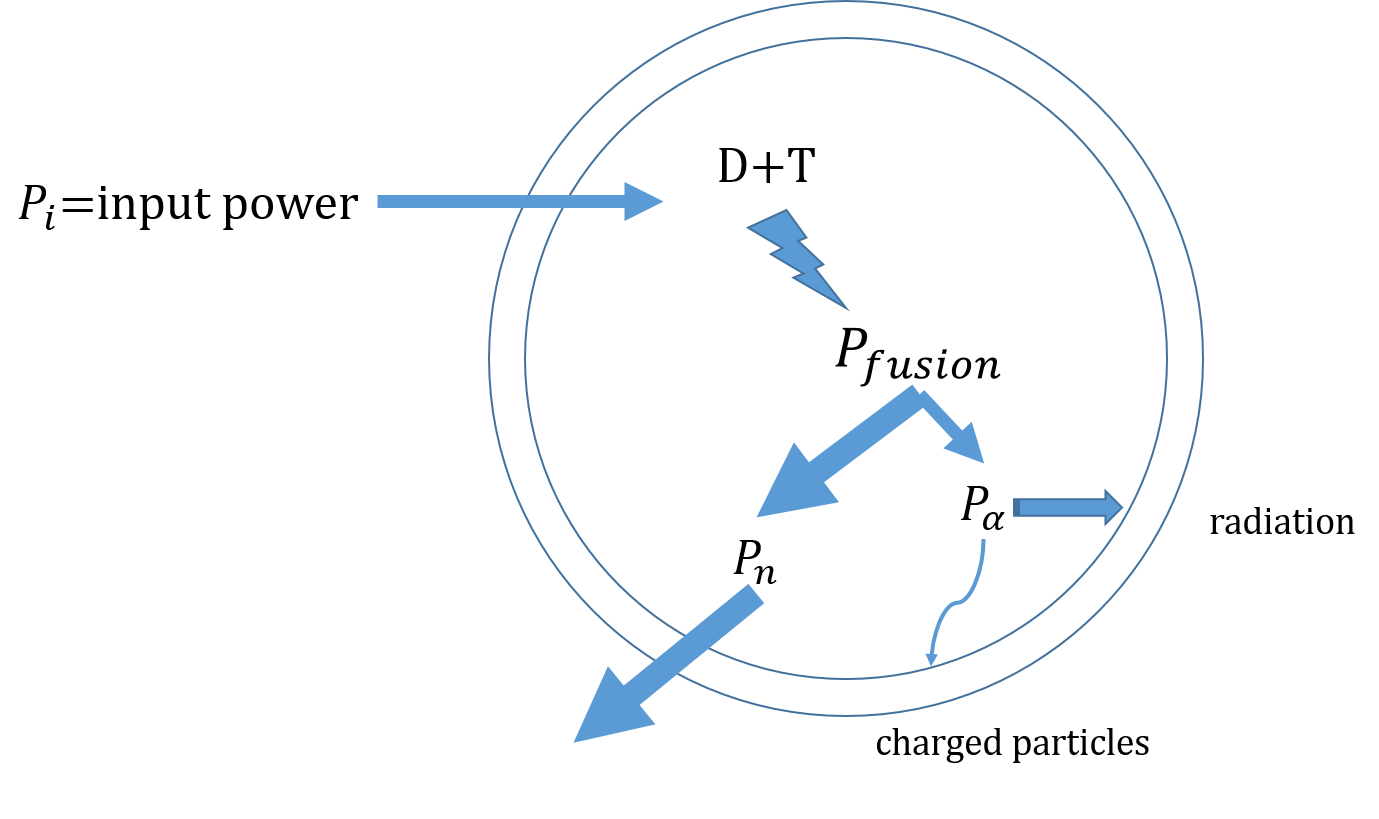
\includegraphics[width=0.75\textwidth]{../images/power_partition.png} 
\caption{Showing a simple partitioning of powers inside a fusion reactor}
\label{fig:power_partition}
\end{figure}

The radiated power goes to the first wall (approximately uniformly) and to surfaces exposed to the plasma ({\it e.g.} limiter). Approximately all the charged particle power is focused to hit the limiter and divertor plate. The partitioning of the $\alpha$-power (and input power) between charged particles and radiation can be controlled to some extent. The control happens via such things as injection of heavy impurities into the plasma to enhance radiation. The balance is expressed as
\begin{equation}
P_\alpha + P_i = P_{rad} + P_{part.}
\end{equation}

The surface heat flux at the first wall is
\begin{equation}
q_{fw} = \cfrac{P_{rad}}{A_w}K_{fw}
\end{equation}
where $K_{fw}$ is a peaking factor for the first wall. Then the surface heat flux to the divertor and limiter is
\begin{equation}
q_{div} = \left( \cfrac{P_{rad}}{A_\text{div}}K_{\text{div}}\right) + \left( \cfrac{P_{part}}{A_\text{div}}K_{\text{div}}\right)
\end{equation}
where $K_\text{div}$ is the peaking factor on the divertor.

{\it Example}:
The STARFIRE-type tokamak with $P_{nw}$ scaled up to 5 MW/m$^2$ has a first wall surface area of 776 m$^2$. The $\alpha$-power is
\begin{align*}
P_\alpha &= P_n \cfrac{3.52}{14.06}\\
& = 5 \times 776 \times \cfrac{3.52}{14.06}\\
& = 971~\text{MW}
\end{align*}

Assuming that 40\% of the $\alpha$ power is radiated to the first wall, we find the average surface heat flux at the first wall as
\begin{align*}
q_{fw} &= \cfrac{971}{776}\times 0.4\\
& = 0.5~\text{MW/m$^2$}
\end{align*}
Which is a very large heat flux! 

Assuming the limiter has a surface area of about 70 m$^2$, the average surface heat flux on the limiter is then
\begin{align*}
q_\text{lim} &= \cfrac{971}{70}\times (1-0.4)\\
& = 8.3~\text{MW/m$^2$}
\end{align*}



%~~~~~~~~~~~~~~~~~~~~~~~~~~~~~~~~~~~~~~~~~~~~~~~~~~~~~~~~~~~~~~~~~~~
\chapter{Nuclear Design of the Blanket}
\label{blanketDesign}
The blanket contains:
\begin{enumerate}
\item Tritium breeding material (lithium in some form)
\item Attenuating materials
\item Neutron multipliers (in some designs)
\item Coolant
\item Structural material
\item Reflector
\item Insulators (in some designs)
\end{enumerate}

The function of the blanket is to convert the kinetic energy of neutrons and $\gamma$-rays into heat, then to transport that heat out of the blanket. The blanket must also breed tritium then facilitate the removal of tritium from the blanket and into tritium processing systems.

\subsection{Schematic of an example blanket}
In Ch.~\ref{intro}, we drew a schematic of a blanket's components in Fig.~\ref{fig:reactor_components}. 

{\it Discussion}: What are the functions and candidate materials in each region?





\section{Tritium breeding}
Lithium is the only material that can provide adequate tritium breeding. The natural abundances of lithium isotopes are
\begin{align*}
^6\mathrm{Li} &\rightarrow 7.42\% \\
^7\mathrm{Li} &\rightarrow 92.58\%
\end{align*}
{\it Discussion}: The two reactions are given in Table~\ref{tab:reactions2}. Which reaction is endothermic? Which is exothermic? What impact will that have on cross-sections and reaction thresholds?


\begin{figure}
\centering
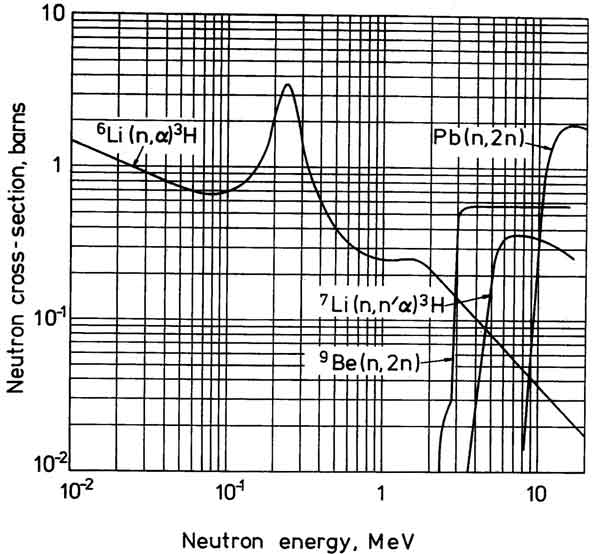
\includegraphics[width=0.8\textwidth]{../images/breeding_xsecs} 
\caption{Cross-sections of various blanket materials. Note the threshold for the $^7$Li and neutron multiplying reactions.}
\label{fig:xsects}
\end{figure}



\subsection{Tritium breeding ratio}
The tritium breeding ratio is defined as 
\begin{equation*}
T = \cfrac{\text{Rate of tritium generation}}{\text{Rate of tritium consumption}} = \cfrac{\dot{N}^+}{\dot{N}^-}
\end{equation*}
where $\dot{N}^+$ is the number of tritium atoms generated per unit time and $\dot{N}^-$ are the number of tritium atoms consumed per unit time.

For a DT cycle, $\dot{N}^- = $~number of fusion reactions in a plasma per unit time (each fusion reaction produces a single neutron). Therefore, for a DT cycle, we have a simplified definition for the tritium breeding ratio.

\begin{equation*}
T = \cfrac{\text{number of tritium atoms produced in the blanket}}{\text{fusion neutron}}
\end{equation*}

If lithium is the breeding material, this can be partitioned as

\begin{equation}
T = T_6 + T_7
\end{equation}
where $T_6$ is the contribution from $^6$Li and $T_7$ is the contribution from $^7$Li.

We define another value as the breeding gain, $G$,

\begin{equation}
G = T - 1
\end{equation}

\subsection{Energy multiplication}
There are many exothermic and endothermic reactions. The total energy deposited in the blanket may be greater or less than the initial kinetic energy of the neutrons (14.06 MeV). Review Table~\ref{tab:reactions2} for the Q values of the lithium reactions.

For reference, the effects of a 30\% lithium enrichment on the Q values are given in Fig.~\ref{fig:enrichment_energy_multiplication}. This table is taken from Ref.~\cite{Abdou1975} to which you may refer for more information. 

\begin{figure}[hb!]
\centering
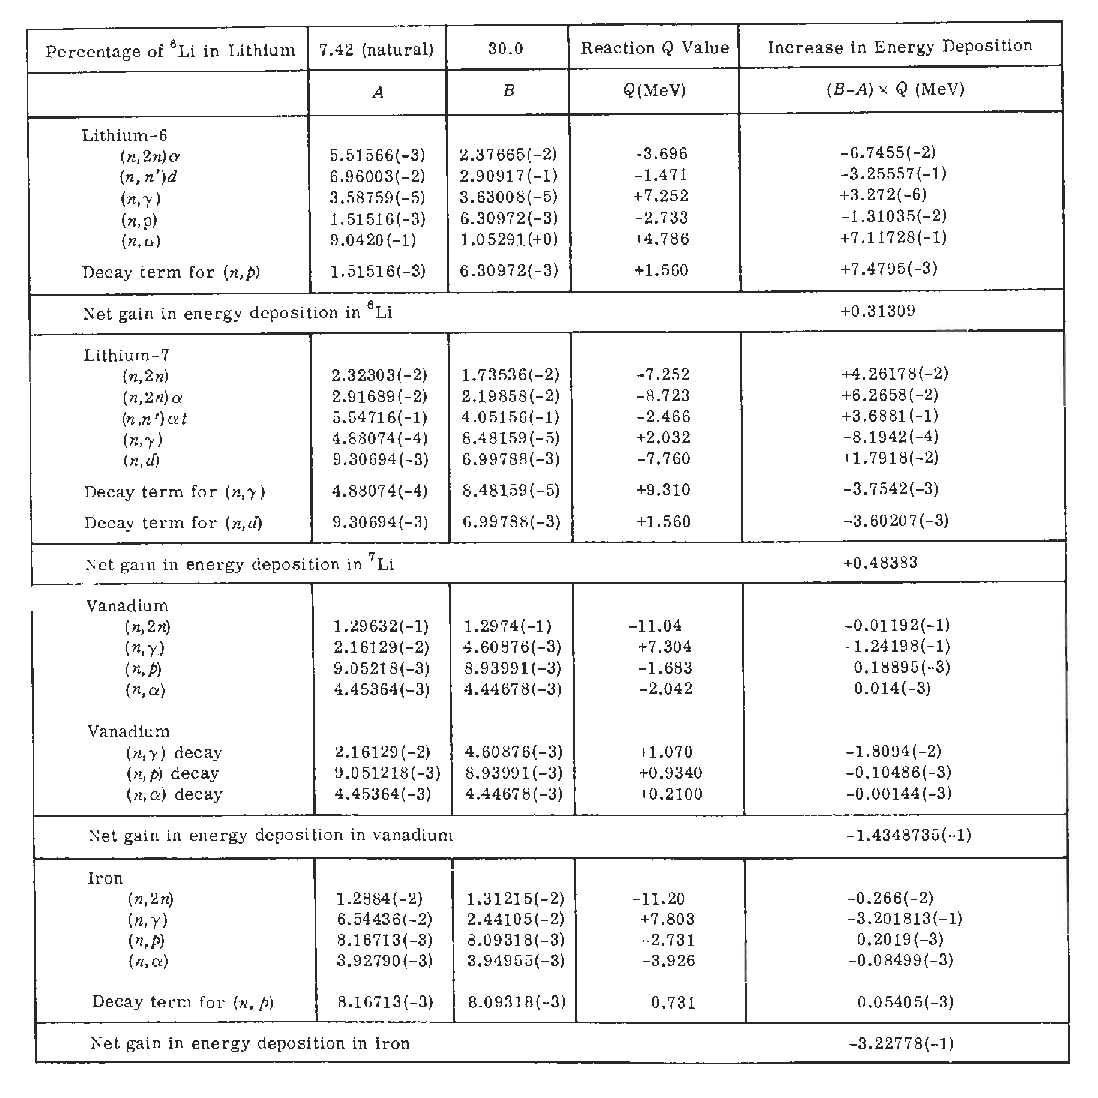
\includegraphics[width=\textwidth]{../images/enrichment_energy_multiplication.eps} 
\caption{Effect of $^6$Li enrichment on reaction rates and energy multiplication. The reaction rates, A and B, are in units of reactions per one fusion neutron.}
\label{fig:enrichment_energy_multiplication}
\end{figure}

We define $E$ as the total energy produced in the system per fusion reaction. This leads to

\begin{align}
E &= \text{Energy generated by neutrons (plus $\gamma$-rays)} + \text{energy due to $\alpha$s} \nonumber\\
& = 14.06 \epsilon + 3.52 \text{ MeV}
\end{align}

where $\epsilon$ is the energy multiplication factor.

\begin{equation}
\epsilon = \cfrac{\text{nuclear energy (in MeV) deposited into the blanket per fusion neutron}}{14.06~\text{MeV}}
\end{equation}

\section{Form of lithium}
Lithium can exist in the breeding blanket as either a liquid or a solid. In current liquid designs, the lithium is often mixed with either lead (17Li-83Pb) or molten salts (LiF-BeF$_2$, LiCL-KCL, LiCL-PbCl$_2$). As a solid, the lithium is mixed with inter-metallic or nonmetallic compounds. As of 2014, most parties researching solid breeder devices are focusing on lithium orthosilicate (Li$_4$SiO$_4$) or lithium metatitanite (Li$_2$TiO$_3$) as candidate ceramics.
\subsection{Designs of lithium-based breeders}
As mentioned, all current designs are either based on liquid or solid forms of tritium. In these categories, there are then different designs that will be explained here.
\subsubsection{Liquid breeders}
Liquid breeders are separated into being either self-cooled or separately cooled. Self-cooled breeders rely on lithium or a lithium-lead (or molten salt) to be both breeder and coolant. Separately cooled breeders have a slow-moving liquid lithium that are responsible only for breeding tritium while a coolant is used ({\it e.g.} helium) to maintain temperature envelopes. Schematics of the two are given in Figs.~\ref{fig:selfCooled} and~\ref{fig:separateCooled}.
\subsubsection{Solid breeders}
Solid breeders are always separately cooled by either water or helium flowing through coolant channels. 

\begin{figure}
\centering
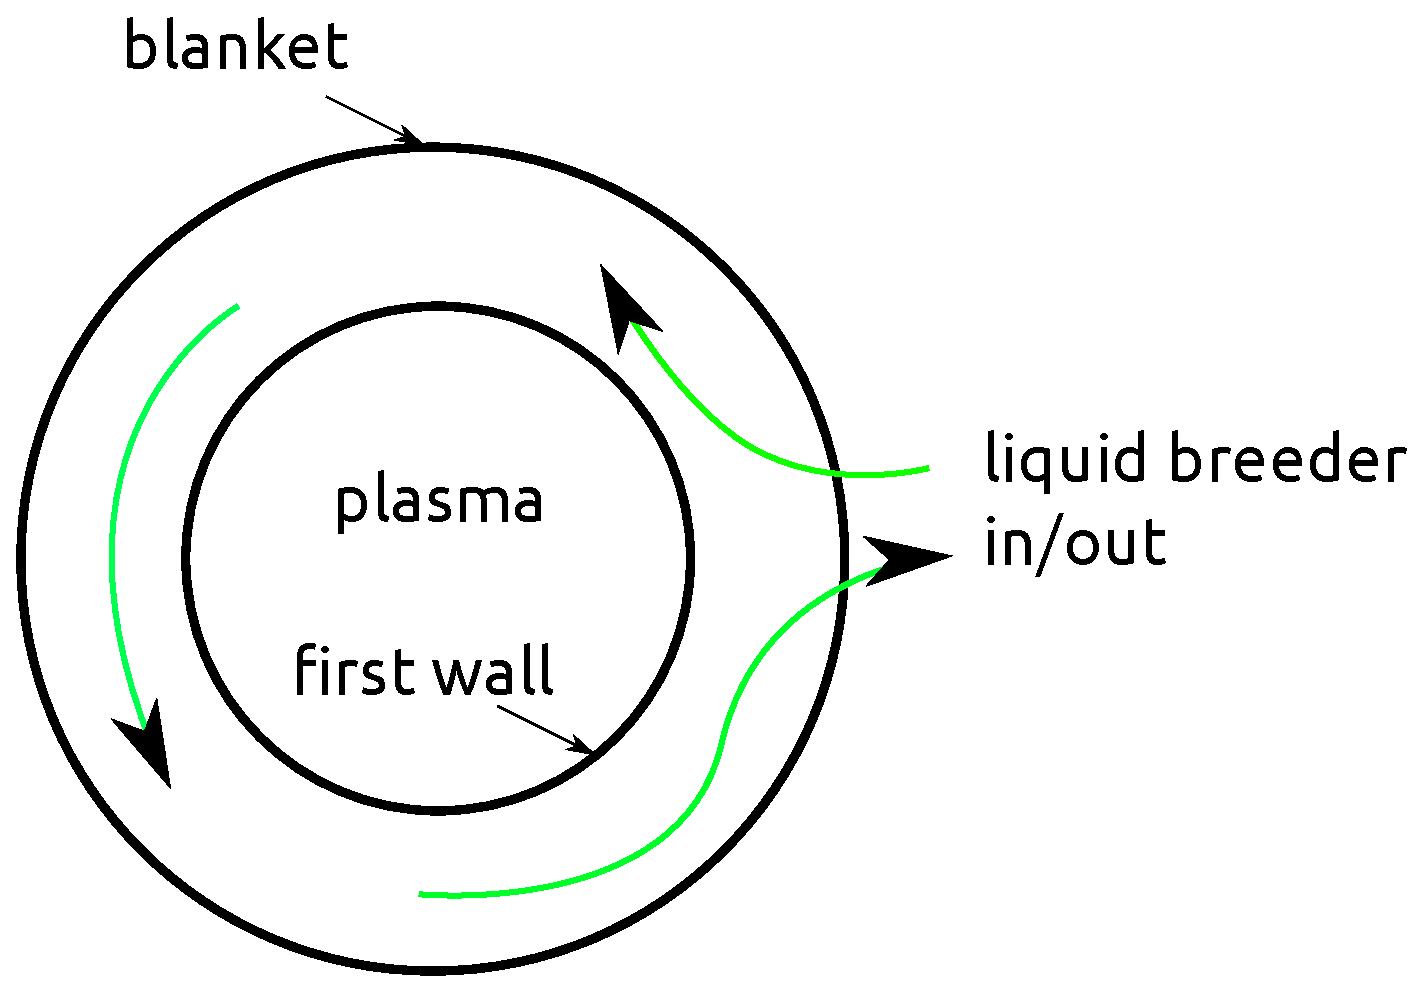
\includegraphics[width=0.65\textwidth]{../images/simplified_self_cooled.eps} 
\caption{Sketch of the liquid breeder acting as a self-cooled device. The flowing lithium produces tritium as well as acts as heat transfer liquid.}
\label{fig:selfCooled}
\end{figure}
\begin{figure}
\centering
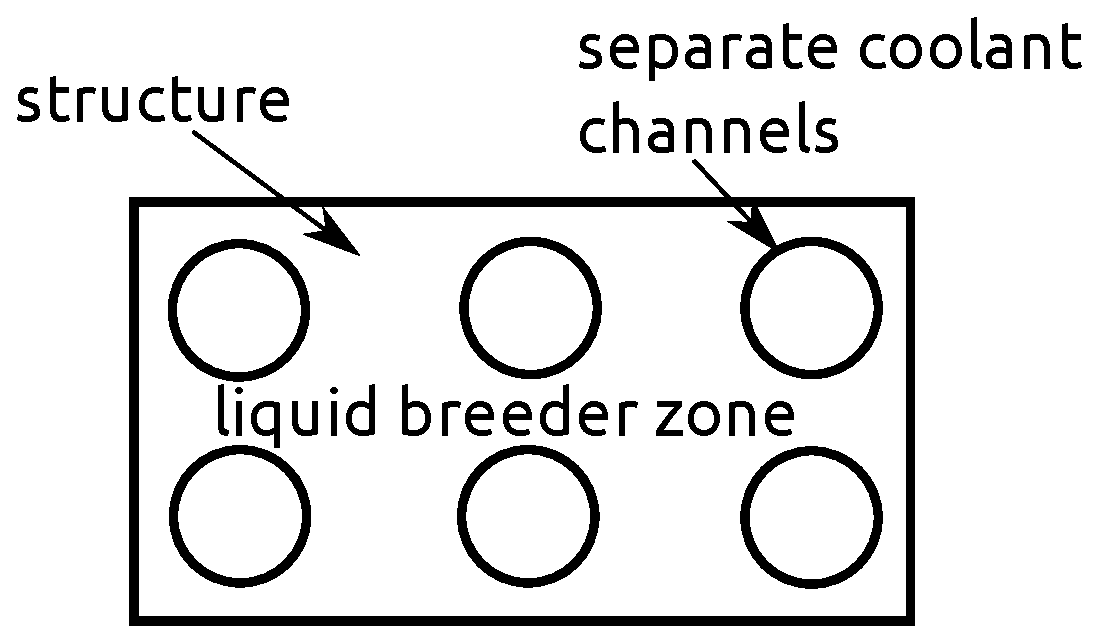
\includegraphics[width=0.5\textwidth]{../images/simplified_separately_cooled.eps} 
\caption{Sketch of the liquid breeder with separate coolant. The stationary breeding zone is cooled separately (typically helium).}
\label{fig:separateCooled}
\end{figure}
\section{Breeding materials}
Because it isn't planned to use pure lithium alone in either blanket concepts, when mixing it with other elements there are certain desirable characteristics it should have, some are:
\begin{itemize}
\item Desirable neutronics characteristics to permit achieving the required breeding ratio
\begin{itemize}
\item High lithium atom density per unit volume
\item Minimum non-lithium atoms; if they are used they should have low scattering and low absorption.
\end{itemize}
\item Should have desirable irradiation characteristics and chemical stability at operating temperatures
\item Should be compatible with other blanket materials
\item Should be able to release tritium ({\it i.e.} tritium inventory should be minimized)
\end{itemize}
\subsection{Lithium}
Some approximate properties of lithium:
\begin{align}
\text{Melting point} & = 180~^\circ C\\
\text{Boiling point} & = 1342~^\circ C\\
N & = 4.2\times10^{22} ~\text{atoms/cm$^3$}\\
k_l & = 50 ~\text{W/m-K}\\
k_s & = 85~\text{W/m-K}
\end{align}
Advantages of lithium
\begin{itemize}
\item yields reasonable breeding ratio (no non-lithium atoms) at natural enrichment without the need for a neutron multiplier.
\item Excellent heat transfer characteristics allowing lithium to serve as both breeder and coolant
\item Tritium recovery is not difficult
\end{itemize}




Disadvantages of lithium
\begin{itemize}
\item {It is chemically active meaning safety is an issue. As an example, here are two reactions with oxygen along with their heats of formation
\begin{align*}
2\mathrm{Li} + \frac{1}{2}\mathrm{O} &\rightarrow \mathrm{Li}_2\mathrm{O} - 142.75~\text{kCal/mol}\\
2\mathrm{Li} + \mathrm{O} &\rightarrow \mathrm{Li}_2\mathrm{O}_2 - 151.9~\text{kCal/mol}
\end{align*}
note: a negative heat of formation means an exothermic reaction. Lithium will exothermically react with water (or air, concrete, or any moisture-containing materials) with high amounts of energy released. Of primary concern in lithium fires is the peak flame temperature. This will determine, to a large extent, whether many radioactive species become air-borne by vaporization. The flame temperature depends on many variables. Some investigations found it to be  about 2500 K which would cause some materials to melt but not vaporize.}
\item MHD effects -- liquid metals have high electrical conductivity. In a magnetic field this leads to a $\vec{J}\times\vec{B}$ force. This in turn leads to pressure drops in the magnetic fluid. To overcome the pressure drop requires increased pressurization and pumping power. The increase in pressurization leads to an increase in stresses of the containing structures and pumping power means more leeching of power from the reactor power plant.
\item Liquid metals tend to be corrosive. Corrosion products transport from radioactive structural materials and are carried downstream into sensitive regions.
\end{itemize}
\subsection{Neutron multipliers}
Neutron multipliers are needed to increase the breeding ratio, particularly in lithium compounds ({\it e.g.} Li$_4$SiO$_4$). Moreover they increase energy multiplication. Materials to act as neutron multipliers would be those that have large neutron multiplication cross sections (over large energy ranges). They react with (n,2n), (n,3n), or even (n, fission), however the fission reaction is obviously not desirable in a pure fusion reactor. Furthermore it is desirable that they have low neutron absorption and that they would have a favorable impact on energy multiplication. 

{\it Discussion}: Neutron multiplication reactions such as (n,2n) are always endothermic. What impact would this have on a fusion reactor?

The two most prominently analyzed neutron multipliers for a fusion reactor are beryllium and lead. Beryllium has a very high nuclide density while also being very light, with a high melting temperature, and high thermal conductivity. However it undergoes a 2-$\alpha$ reaction that causes trapped helium to swell the material. There is also a rarely occurring reaction with beryllium that generates tritium; it is frequent enough to cause a concern with contamination.

\begin{thebibliography}{9}

\bibitem{Abdou1975}
  Abdou, M. A. and Maynard, C. W.,
  \emph{Calculational methods for nuclear heating -- part II: Applications to fusion-reactor blankets and shields}.
  Nuclear Science and Engineering,
  1975.

\end{thebibliography}


\end{document}